The ETD 2024 conference activities will be held at Avani Victoria Falls' \textbf{Convention Centre}.

\textbf{Tea/Coffee breaks and lunches} will be offered during the conference.

The \textbf{poster session} will be held on Wednesday, November 6 2024 and will comprise of a \textbf{"one minute madness"}, followed by a textbf{Poster Session with Tea/Coffee}.

Wi-Fi will be available during the conference. The Zambia Research and Education Network will also provide access to an eduroam network throughout the duration of the conference.

The \textbf{conference welcome reception} will be held at the \textbf{Mukuni BOMA Village}, on the banks of the Zambezi River.

\section{How to get to the Avani Victoria Falls Resort?}

Avani Victoria Falls Resort is located on the banks of the Zambezi river with a 5-minute walk direct access to Victoria Falls.

\begin{itemize}

	\item \textbf{Air:} From Lusaka, Kenneth Kaunda International Airport, you can fly directly to Livingstone, Harry Mwaanga Nkumbula International Airport (formerly known as Livingstone Airport). Flights are available with Proflight Zambia (daily flights) or Zambia Airways (daily flights). The journey takes around 1 hour and 10 minutes. Harry Mwaanga Nkumbula International Airport in Livingstone also has direct flights from Johannesburg (JNB), Cape Town (CPT) and Nairobi (NBO), (South Africa and Kenya). Note that the most frequent flights to Livingstone are routes from Lusaka (LUN), domestic, and Johannesburg (JNB), South Africa, with an average of 6 flights per day.
	\item \textbf{Bus:} Various long-distance buses operate daily between Lusaka and Livingstone. Buses leave Lusaka from 6:00 am and every half hour thereafter until 11.30 am. The journey takes around 6 to 7 hours.
	\item \textbf{Getting Around:}
	\begin{itemize}
	    \item \textbf{Taxis}: Taxis are readily available and can be hired for specific trips, for a half-day or for a full-day.
        \item \textbf{Local mini-buses}: There is a network of local mini buses that connect various parts of Livingstone.
    \end{itemize}
	
\end{itemize}

\subsection{Avani Victoria Falls Resort: Google Maps Location}

\begin{center}
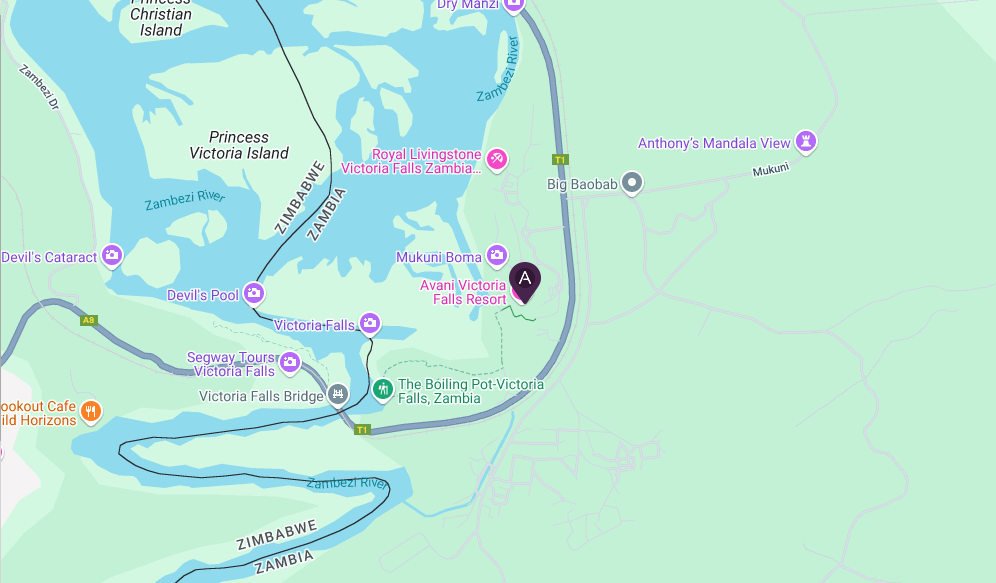
\includegraphics[width=\linewidth]{images/img-etd24-avani_victoria_fall_convention_centre_map.png}
\end{center}


\subsection{Avani Victoria Falls Resort: Convention Centre Layout}

\begin{center}
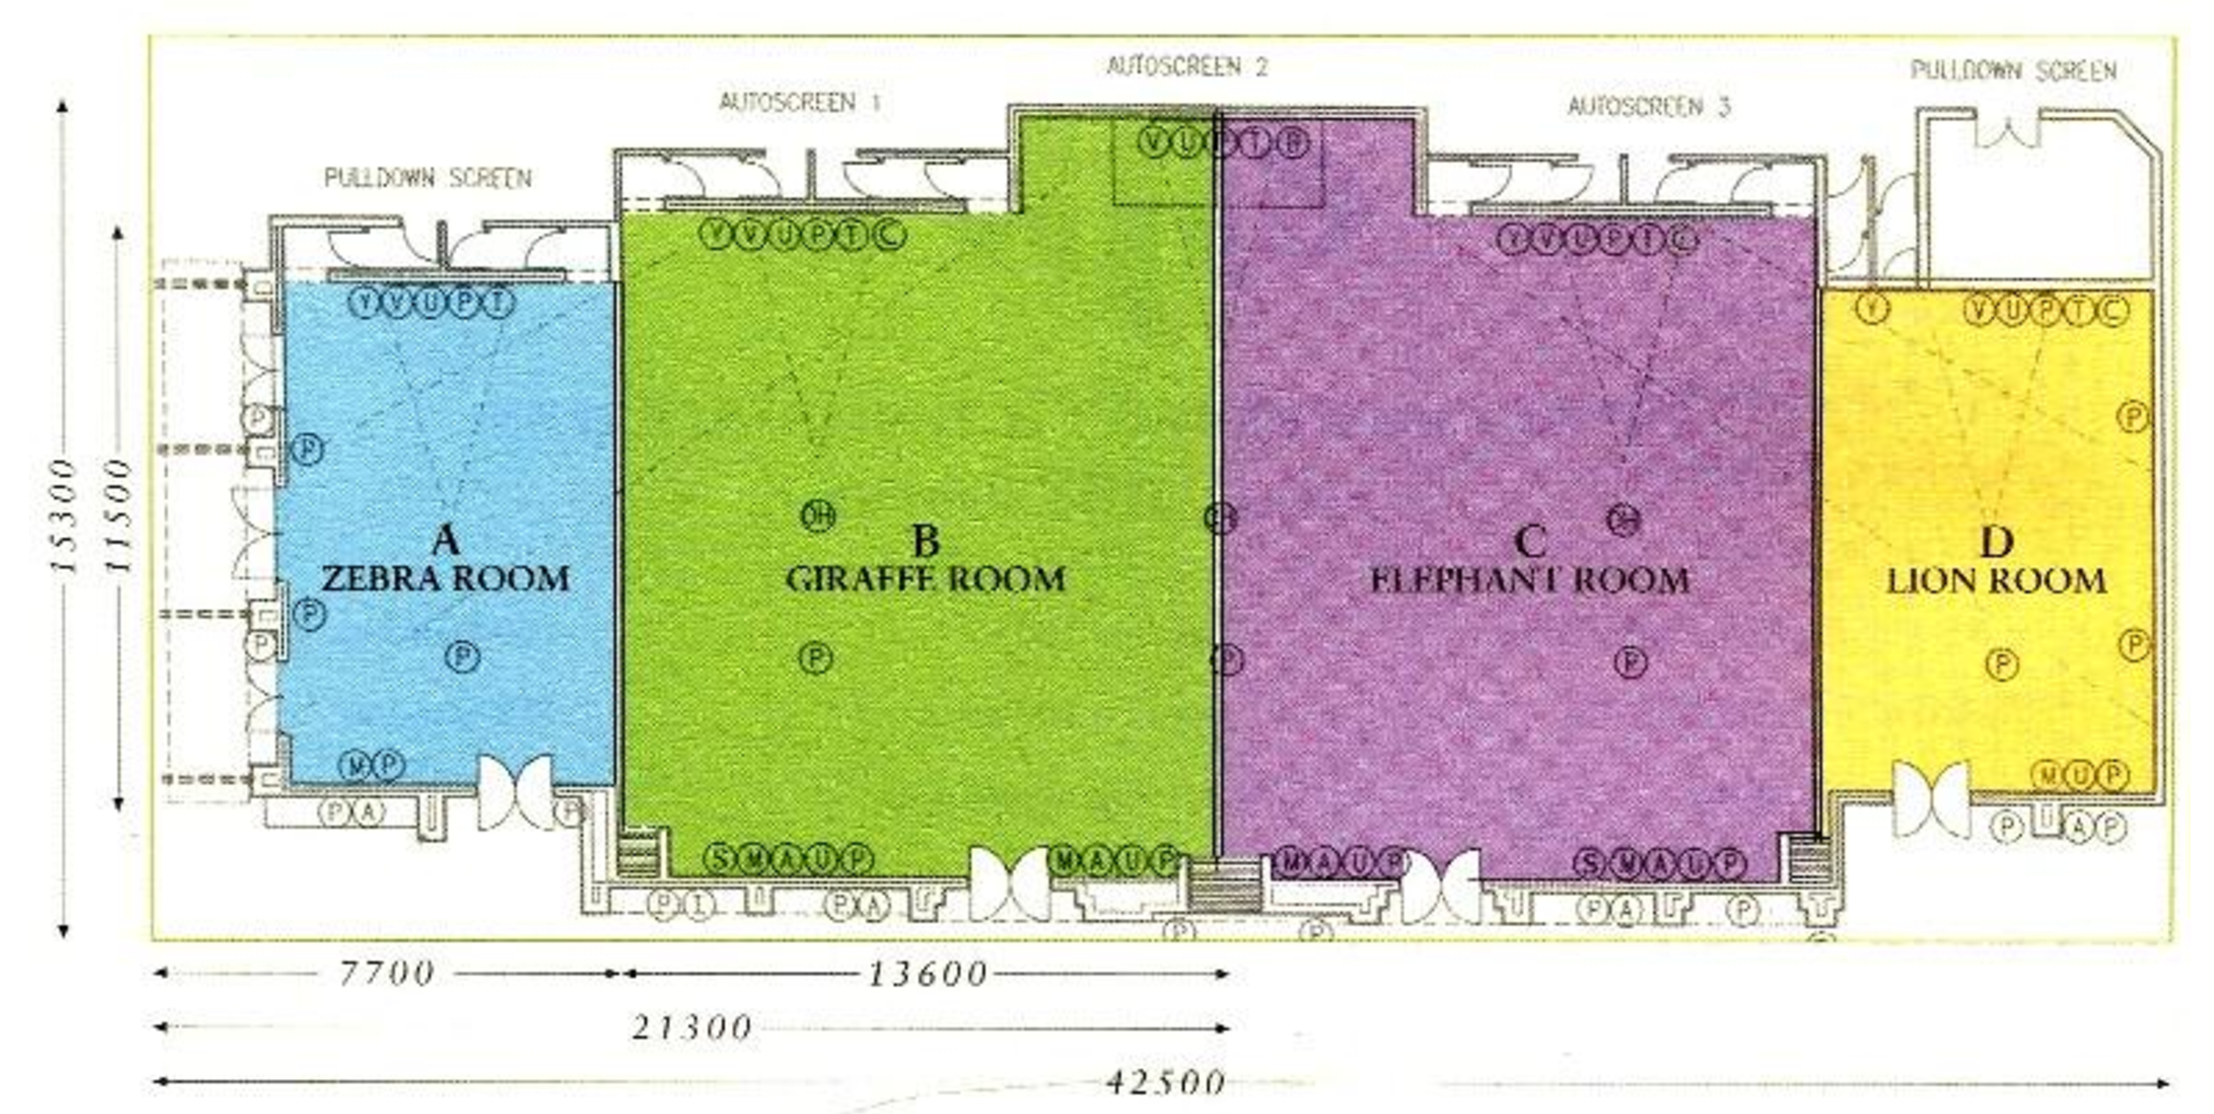
\includegraphics[width=\linewidth]{images/img-etd24-avani_victoria_fall_convention_centre_layout.png}
\end{center}
